\pdfoutput=1
\documentclass[pra,twocolumn,showpacs,amsmath,amssymb, aps, 10pt]{revtex4-1}

\usepackage{graphicx}%Include figure files
\usepackage{dcolumn}%Align table columns on decimal point
\usepackage{bm}% bold math
\usepackage{placeins}
\usepackage{subcaption}
% \usepackage[page]{appendix}

\graphicspath{{../images/}}

%\nofiles

\begin{document}

\title{Project 2: Chaos in 1-D Scattering}


\author{John Russo}
\affiliation{Department of Physics and Astronomy, University
of Delaware, Newark, DE 19716-2570, USA}

\begin{abstract}
  In this paper, the emergence of chaotic motion in a one-dimensional system of
  two colliding balls is studied. The balls
  move under the influence of gravity, and are subject to elastic collisions with each
  other and the floor. Collision and bounce times are computed, and the trajectories
  sampled in the intervals between these events. By varying initial positions,
  velocities, and the mass ratio $m_2/m_1$ of the two balls, the parameter space where chaotic motion
  appears is explored. This motion is characterized through trajectories of the balls,
  and
  Poincare sections, autocorrelation and the Lyapunov exponent of the top ball's trajectory.
  It is found that the setting $m_2/m_1=1$ yields nonchaotic motion, $m_2/m_1=9$
  can produce both nonchaotic and chaotic motion, and $m_2/m_1=0.5$ results in
  strongly chaotic motion. This shows that a relatively simple system can exhibit
  a diverse range of dynamical behavior by modifying initial conditions.
\end{abstract}

\pacs{45.40.Aa} %Translational kinematics


\maketitle

\section{Introduction} \label{sec:intro}

Classical systems that obey certain criteria can exhibit chaotic behavior, where
slight changes in initial conditions produce exponential divergence in behavior.
In other words, chaotic systems exhibit extreme sensitivity in initial
conditions.\cite{taylor}

In order to be chaotic, a system must exhibit:
\begin{enumerate}
  \item nonlinearity, \label{nonlinearity}
  \item dependence on more than three variables, and \label{dependence}
  \item sensitivity to initial conditions. \label{sensitivity}
\end{enumerate}

These conditions are necessary, but not sufficient to produce chaotic behavior.
A system can be chaotic for certain initial conditions but not others, as shown
in Section~\ref{sec:partially_chaotic} below.

In this paper, behavior of the one-dimensional system of colliding balls shown
in Fig.~\ref{fig:balls} is studied.
The balls are modelled as points which can elastically collide with each other
and with the floor. Dynamical equations of motion governing both the trajectories
of the balls and collisions between them are discussed
in Section~\ref{sec:methods}.

\begin{figure}[h]
  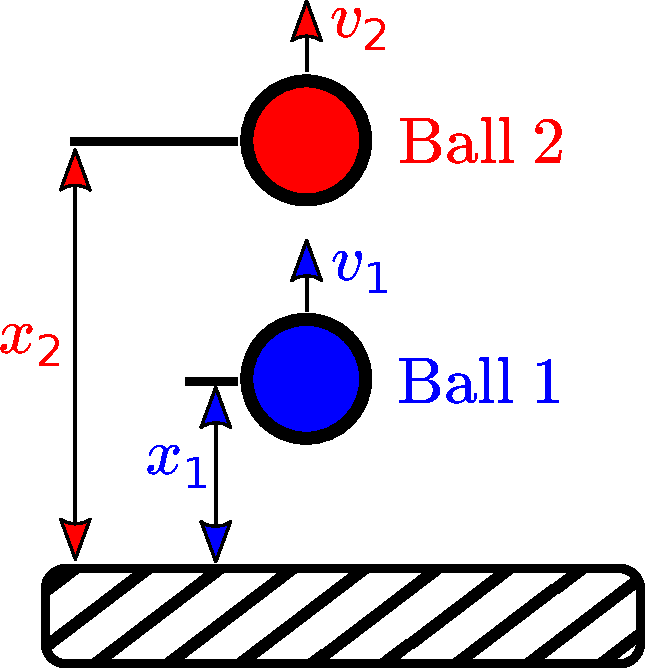
\includegraphics[width=.8\linewidth]{balls}
  \caption{Diagram of the one-dimensional system of balls simulated in this
  paper. The element at the bottom represents the floor upon which the bottom
  ball bounces.}
  \label{fig:balls}
\end{figure}

By varying parameters of the system such as the relative masses of the balls and
the initial positions and velocities of the balls, a wide range of dynamical
behavior is exhibited. Of particular interest are the chaotic modes, where
minor variance in initial conditions causes exponential divergence in the positions
of the balls. The lens this system gives us into how varying initial
parameters is of particular interest for modelling and analysis to further
understand chaos.



\section{Methods} \label{sec:methods}

The system studied in this paper consists of two balls subject to gravity and
collisions with each other and the ground. The term \textbf{event} will be used
to refer to both collisions between the balls and bounces of ball 1
off the floor. Between events, each
ball obeys the one-dimensional kinematics equation

\begin{equation}
  x(t) = x_0 + v_0 t + \frac{1}{2} g t^2
  \label{eq:kinematics}
\end{equation}

where $x_0$ and $v_0$ refer to the position and velocity
of the ball after the previous event, $x$ is the position of the ball,
$g$ is the acceleration due to gravity, and $t$ is the time since the previous
event. %TODO: Repetitive phrasing here, also run-on of the ages

The normalization used is defined by
\begin{align}
x' &= \frac{mg}{E} x \\
v' &= \sqrt{\frac{m}{E}} v \\
t' &= \sqrt{\frac{mg^2}{E}} t \\
E &= \frac{1}{2} m_1 v_1^2 + \frac{1}{2} m_2 v_2^2 + m_1 g x_1 + m_2 g x_2
\label{eq:normalization}
\end{align}
where $E$ is the energy in non-normalized units.\cite{assignment}

The normalized energy $\bar E$ is therefore defined as
\begin{equation}
  \bar E = 1 = \frac{m_1}{2 m} \bar v_1^2
  + \frac{m_2}{2 m} \bar v_v^2
  + \frac{m_1}{m}\bar x_1
  + \frac{m_2}{m}\bar x_2
\end{equation}
and is conserved.

Primes are used here to explicitly indicate normalized quantities.
In this normalization, $g$ is set to unity, and the equation of motion
Eq.~\ref{eq:kinematics} is written in terms of normalized variables as
\begin{equation}
x'(t) = x'_0 + v'_0 t' - \frac{1}{2} t'^2.
\label{eq:kinematics_normalized}
\end{equation}
Bounces and collisions are both characterized by
 Eqs.~\ref{eq:elastic1}~and~\ref{eq:elastic2} for elastic collisions, in which
the total energy is conserved.

Henceforth, quantities in this paper are assumed to be normalized by this convention
unless explicitly labeled with a unit.


\subsubsection{Trajectory analysis algorithm}

The algorithm used to numerically evaluate the system follows a two-fold approach
to exactly solve for the positions of the balls at any time.

First, the positions, velocities, and times of each event are
computed sequentially.
Beginning with the initial conditions, the times for each
ball to reach the ground are computed. If the second ball would reach the ground
before the first, then a collision must occur before the first ball reaches the
ground. The time of this collision is determined by setting the equations of
motion for each ball, given by Eq.~\ref{eq:kinematics_normalized} with the
appropriate initial conditions inserted, equal to each
other and solving for $t$.

If the event is a collision, then the velocities of the balls are updated according
to Eqs.~\ref{eq:elastic1}~and~\ref{eq:elastic2} for elastic collisions.
For balls $1$ and $2$, these are

\begin{align}
  v_{1,f} &= \frac{m_1-m_2}{m_1+m_2}v_{1,i} + \frac{2 m_2}{m_1+m_2}v_{2,i} \label{eq:elastic1}\\
  v_{2,f} &= \frac{2 m_1}{m_1+m_2}v_{1,i} - \frac{m_1-m_2}{m_1+m_2}v_{2,i}
  \label{eq:elastic2}
\end{align}

respectively, where the subscript $i$ indicates the velocity immediately before the collision,
and the subscript $f$ indicates the velocity immediately after.

Bounces can only happen for ball 1. Ball 2 cannot hit the floor, since it would
collide with ball 1 first. If the event is a bounce, then the velocity of ball 1
is inverted so it is then travelling up.

This algorithm continues until the first event outside of the desired maximum
time is detected. In this way, the phase space coordinates and times of each
event are calculated.
This is sufficient to plot Poincare sections, shown for ball 2 in
Section~\ref{sec:results}.

The second stage of the algorithm involves calculating the trajectories of each
ball. This is necessary both for plotting the spatial trajectories, and for
calculating autocorrelations and Lyapunov exponents.

To meaningfully calculate autocorrelations, it is desirable
for the phase space coordinates of each ball to be determined evenly spaced in time.

Recall that between each event, the motion of each ball is given by
Eq.~\ref{eq:kinematics_normalized}. So, the motion is completely determined by
the phase space coordinates of the ball at the previous event, and the time
since that event.

A list of evenly-spaced timesteps at which the trajectories will be sampled at
is generated. For each interval between events, a function of the form
Eq.~\ref{eq:kinematics_normalized} is created, with the initial conditions $x'_0$
and $v'_0$ determined by the phase space coordinates of the previous event, along
with the start and end time of the interval.

Each timestep is iterated over, invoking the appropriate function for the
interval it falls in to evaluate the positions and velocities of the balls.

Further details on optimizations done to this algorithm are available
in Appendix~\ref{appendix:traj}.


\subsubsection{Autocorrelation}

Autocorrelations $a(\tau)$ were calculated for each lag $\tau$ according to
\begin{equation}
  a(\tau) = \frac{1}{N-\tau} \sum_{i=1}^{N-\tau}
  \left(f_i - \bar f \right)
  \left(f_{i+\tau} - \bar f \right)
  \label{eq:acorr}
\end{equation}
where $N$ indicates the total number of lags, $f_i$ is the set of discrete
positions, and $\bar f$ is the mean of $f$. Total number of lags was selected
as $10\%$ of the total number of elements in the dataset.

Since the implementation of this provided acceptable runtimes even over datasets
on the order of hundreds of thousands of elements, no subsampling was performed.


\subsubsection{Lyapunov Exponent}

For a chaotic system, separation between two systems with very similar initial
conditions grows as
\begin{equation}
  | \Delta x(t) | \propto K e^{\lambda t}
\end{equation}
where $| \Delta x(t) |$ is the magnitude of the separation of the two systems,
$K$ is a constant, and $\lambda$ is the Lyapunov exponent.\cite{taylor}

In this system, separation was defined as the difference in ball 2's position
for the two systems. The difference in initial conditions was an increase of
$x_2$ by $10^{-6}$. Plotting this on a log plot shows the exponential nature
of the increase in separation for chaotic systems.


\subsubsection{Simulation Details}

For the simulations performed in this paper, a timestep
of $10^{-2}$ seconds was used for sampling trajectory data. This was found to give
sufficient resolution for generating plots and for calculating autocorrelations and
Lyapunov exponents.


Poincare sections were run for longer times than the plotted trajectories shown
in order to give sufficient density of points to show details of the
chaotic phase space. Since the Poincare sections can be generated
before the trajectories between each bounce are calculated, they could
efficiently be run for much longer times than the trajectories. All plotted
Poincare sections are for the phase space coordinates of ball 2 at the times of
collisions with ball 1.





\section{Results} \label{sec:results}

It is found that the presence of chaotic behavior depends strongly on the
mass ratio $m_2/m_1$ of the two balls. In Sections~\ref{sec:nonchaotic}-\ref{sec:chaotic-2},
this transition from nonchaotic to chaotic behavior is studied for a range of
initial conditions.

For all simulations done, initial conditions are $v_1 = v_2 = 0 \mathrm{m/s}$ and
$x_1 = 1$m, $x_2 = 3$m unless otherwise specified.


\subsection{Nonchaotic}\label{sec:nonchaotic}
Nonchaotic behavior in this system is characterized by periodic, oscillatory motion.
This can be seen for the mass ratio $m_2/m_1 = 1$, where the trajectories of
the balls oscillate roughly periodically as in Fig.~\ref{fig:1-traj}.

The stability of these
modes of oscillation can be better visualized in a Poincare section plotted
for ball 2 at the times of collisions, shown in
Fig.~\ref{fig:1-poincare}. Only two lines in the phase space trajectory
are visible, despite being run for large time.
This indicates that the ball follows a stable path in phase space, which
indicates a nonchaotic system. Examples of chaotic Poincare sections are
shown in Sections~\ref{sec:chaotic-9}-\ref{sec:chaotic-2}, such as in
Fig.~\ref{fig:9-poincare}, and show vastly different qualitative
behavior. More detail is provided on this in those sections.

\begin{figure}
  \begin{subfigure}{0.8\linewidth}
    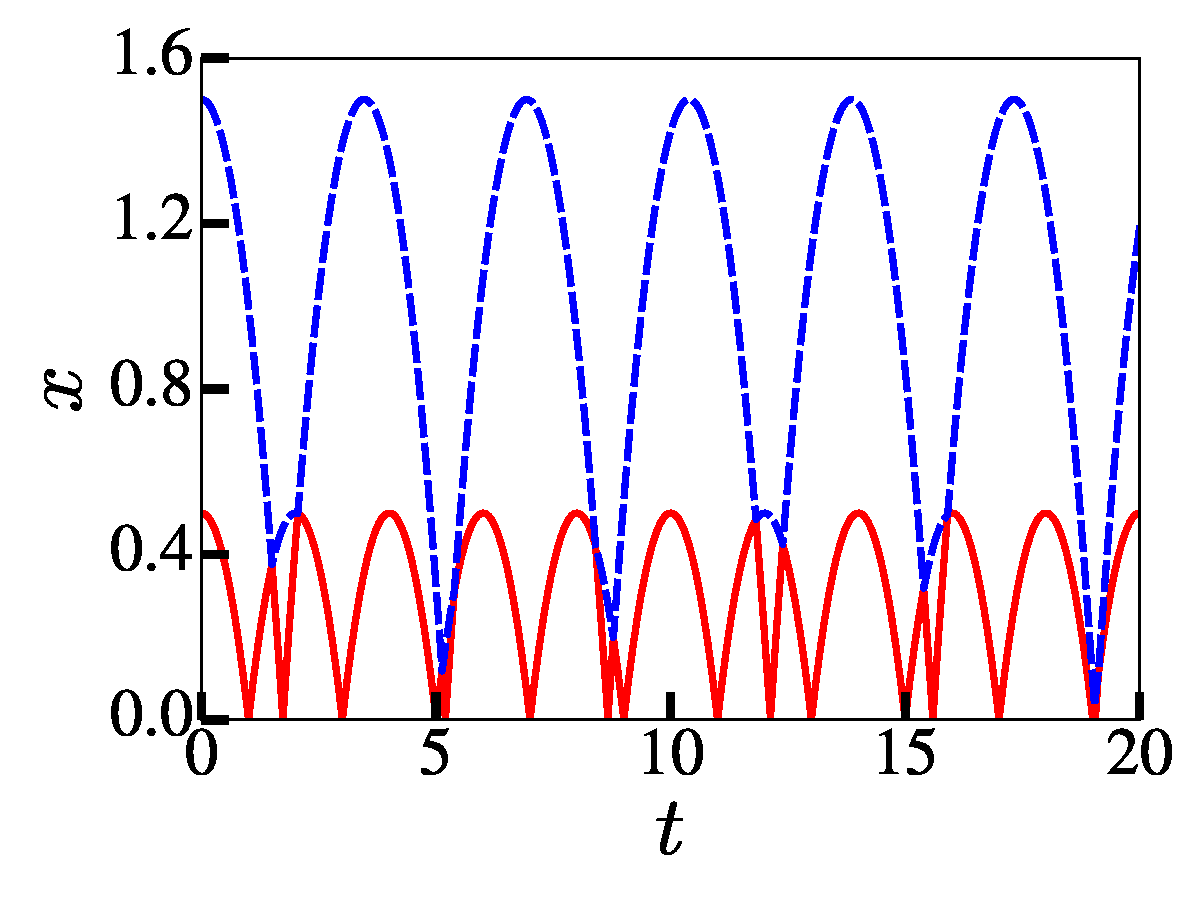
\includegraphics[width=\linewidth]{r1_0_traj}
    \caption{Trajectories of ball 1 (red, solid line) and ball 2 (blue, dashed line).}
    \label{fig:1-traj}
  \end{subfigure}

  \begin{subfigure}{0.8\linewidth}
    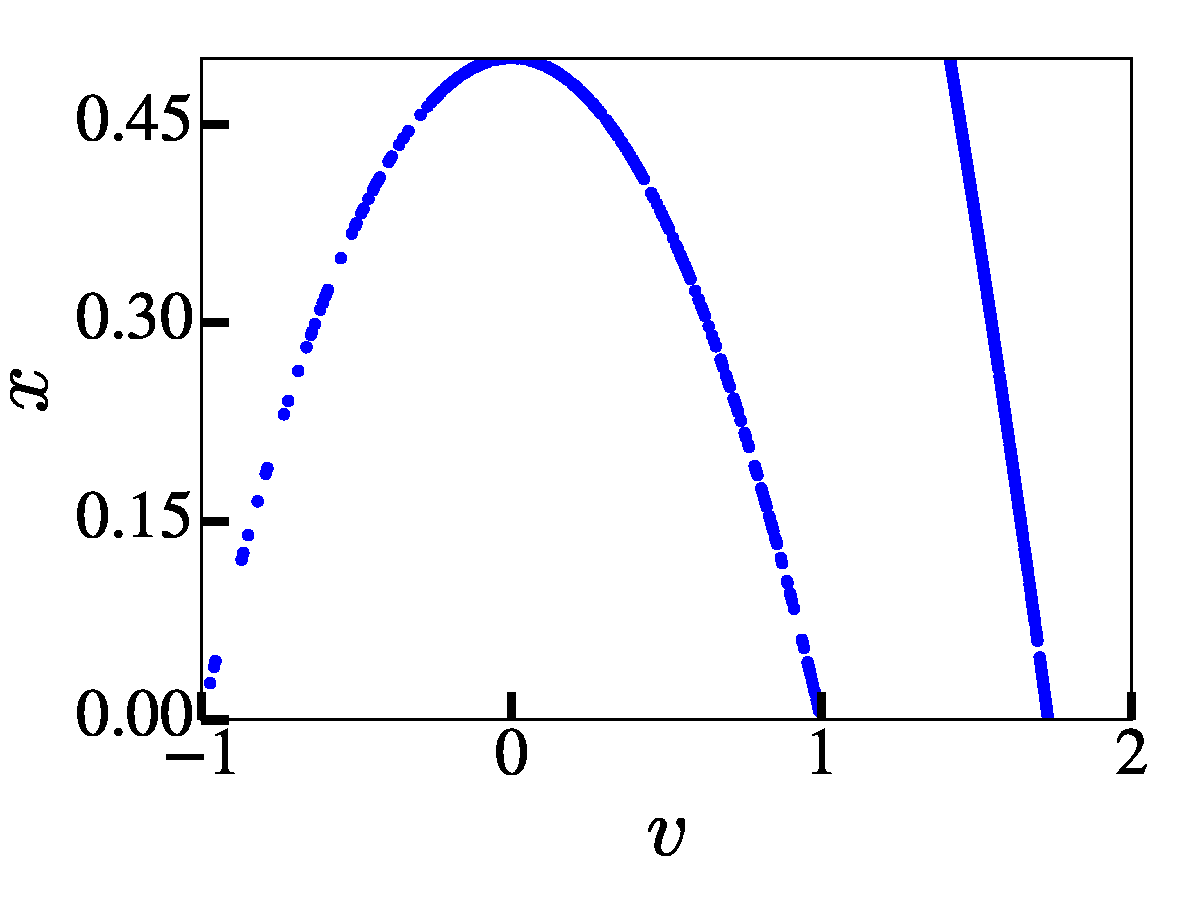
\includegraphics[width=\linewidth]{r1_0_poincare}
    \caption{Poincare section for ball 2,  plotted in phase space for every collision
    between the balls to $t=5000$s, chosen to provide sufficient density of points.}
    \label{fig:1-poincare}
  \end{subfigure}

  \caption{Trajectories and Poincare section for $m_2/m_1 = 1$.}
\end{figure}

\subsubsection{Autocorrelation}

How chaotic these trajectories are can be parameterized by examining autocorrelation
curves, which measure data's self-similarity over time. Nonchaotic motion would
be expected to have strong correlation with itself over time.


\begin{figure}
  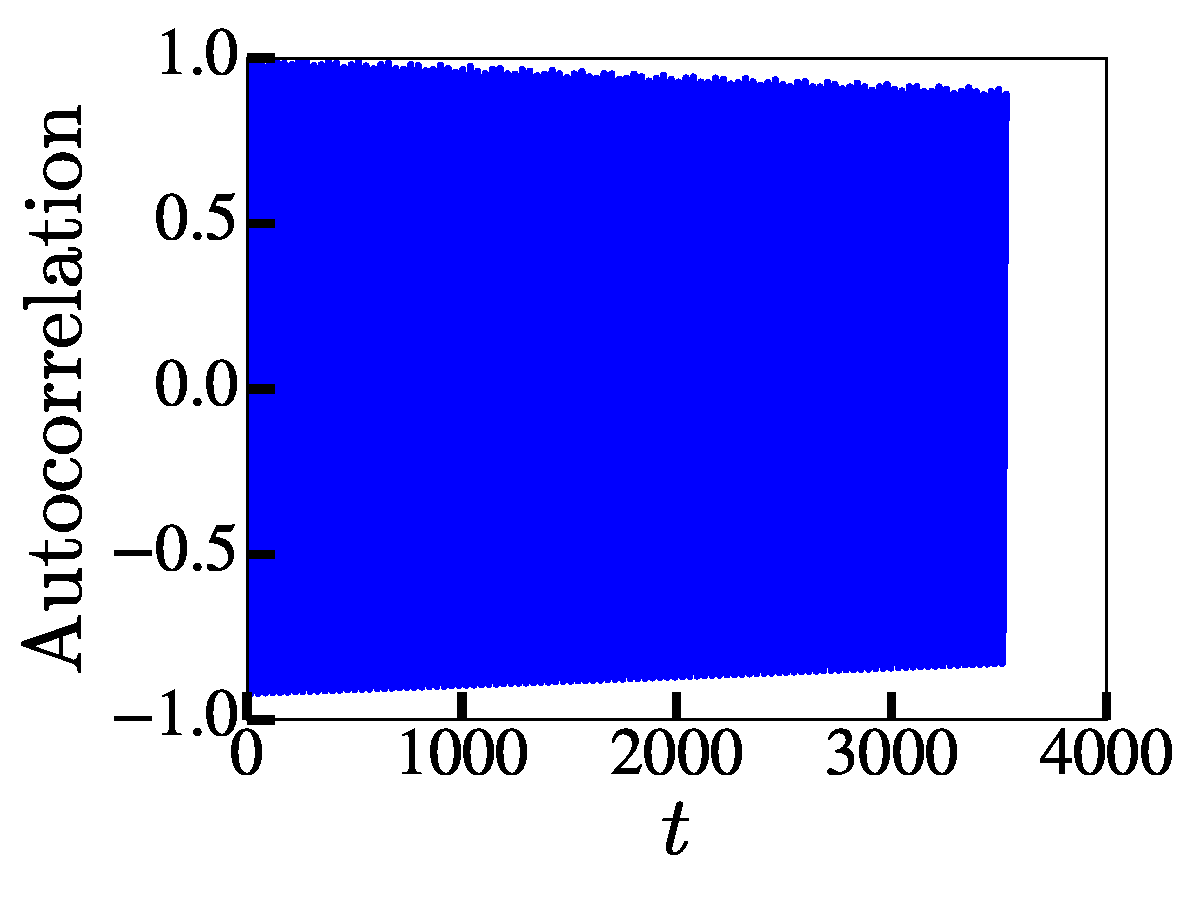
\includegraphics[width=0.8\linewidth]{r1_0_acorr}
  \caption{Autocorrelation for $m_2/m_1 = 1$. The autocorrelation
  rapidly oscillates, which causes it to appear almost solid. Strong
  correlation is present even at long times.}
  \label{fig:1-acorr}
\end{figure}

In Fig.~\ref{fig:1-acorr}, the autocorrelation curve shows strong correlations
even up to times very long compared to the timescales of bounces and collisions.
The autocorrelation is oscillatory, which causes the plot to appear almost solid.
This is expected for a nonchaotic system, and thus confirms that this motion is nonchaotic.


\subsection{Approaching Chaos}\label{sec:partially_chaotic}

To examine how periodic motion begins to transition into aperiodic chaotic motion,
let us now change the mass ratio to $m2/m1 = 9$. This case is particularly
interesting, since certain selections
of initial conditions can recover periodic, nonchaotic behavior.

By setting
$v_1 = 0.879$, the system exhibits the behavior shown in Fig.~\ref{fig:9-nonchaotic}.
Though the spatial trajectories of the balls in Fig.~\ref{fig:9-traj-nonchaotic}
are more complex than the trajectories for the $m_2/m_1 = 1$ case, and in fact
appear almost aperiodic, examining the phase space trajectory shown in
Fig.~\ref{fig:9-poincare-nonchaotic} shows that the motion samples a fixed path
through phase space.

\begin{figure}
  \begin{subfigure}{0.8\linewidth}
    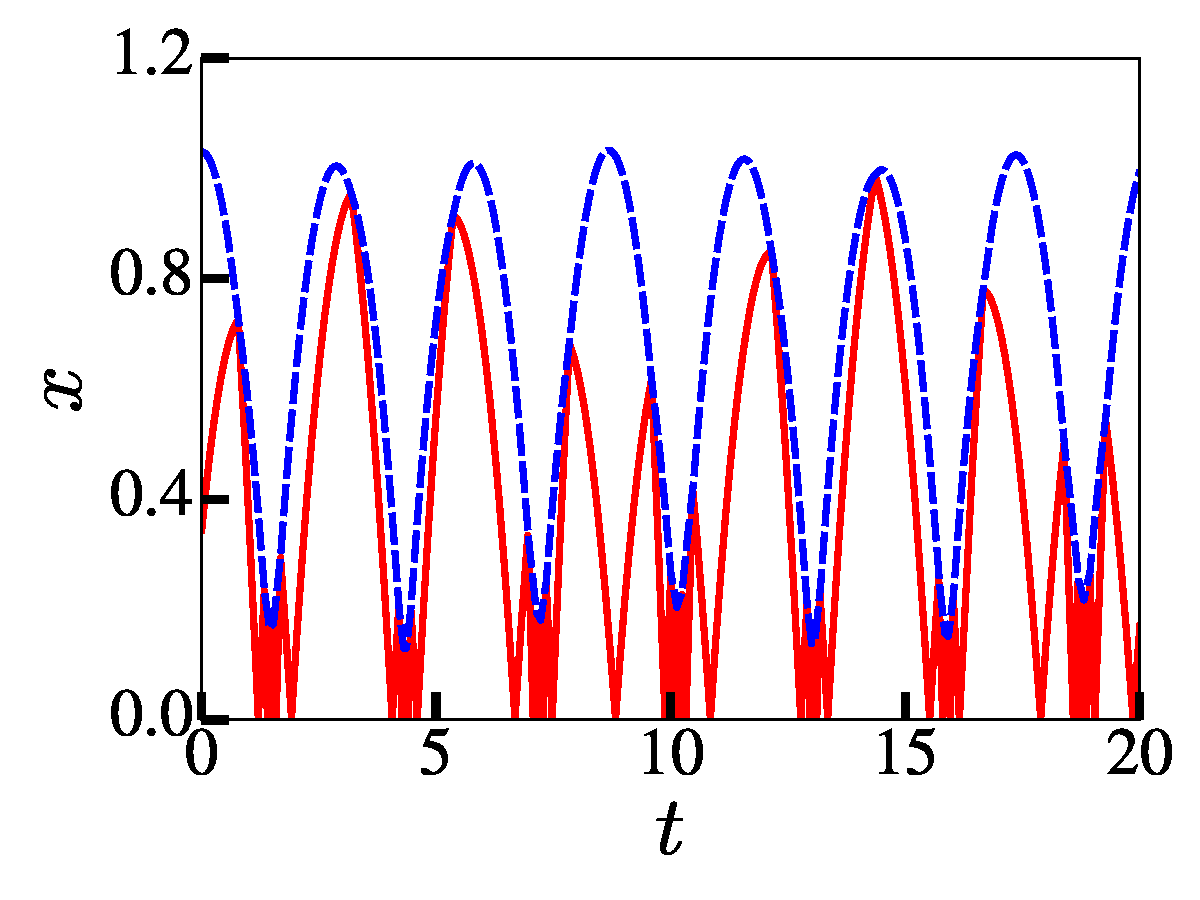
\includegraphics[width=\linewidth]{nonchaotic_r0_1_traj}
    \caption{Trajectories of ball 1 (red, solid line) and ball 2 (blue, dashed line).}
    \label{fig:9-traj-nonchaotic}
  \end{subfigure}

  \begin{subfigure}{0.8\linewidth}
    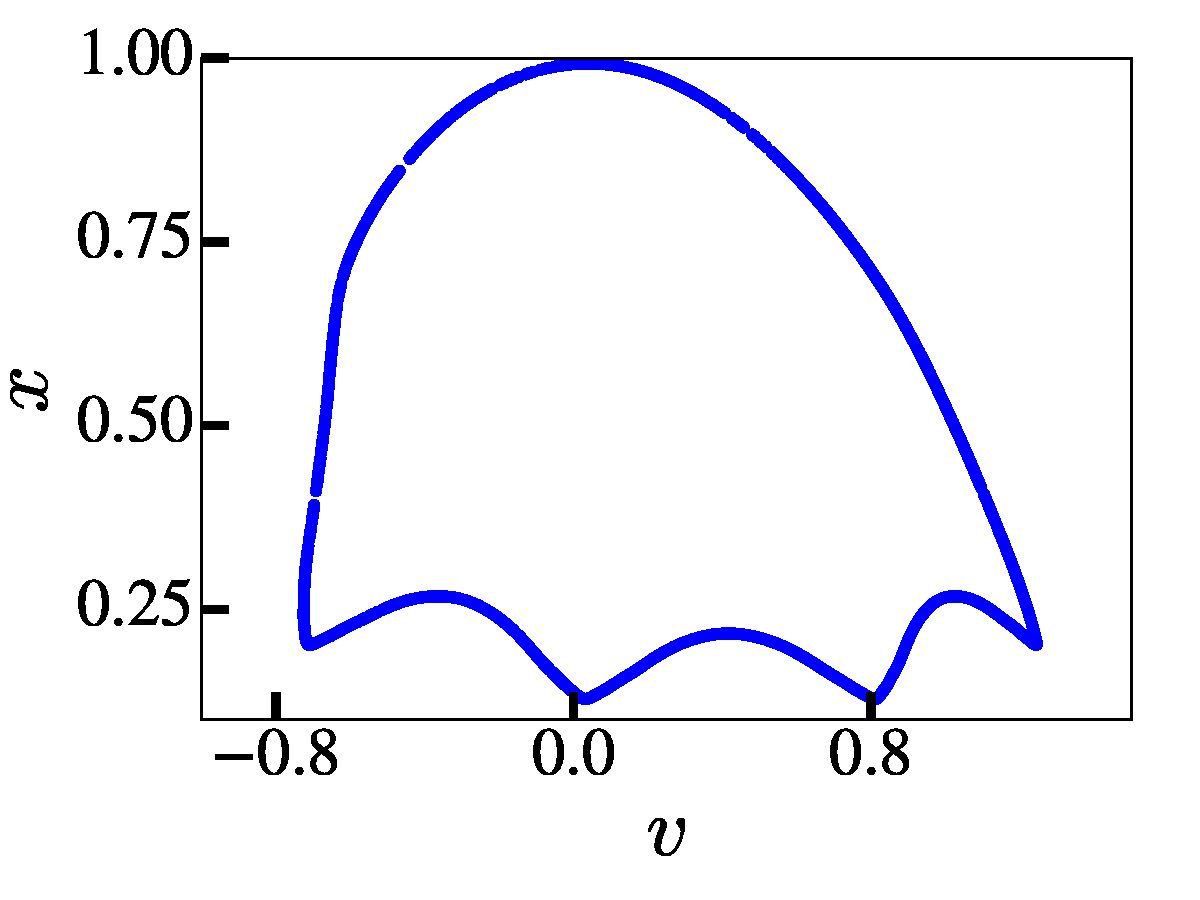
\includegraphics[width=\linewidth]{nonchaotic_r0_1_poincare}
    \caption{Poincare section for ball 2, plotted in phase space for every collision
    between the balls to $t=5000$s. The trajectory through phase space follows a
    closed loop.}
    \label{fig:9-poincare-nonchaotic}
  \end{subfigure}

  \caption{Trajectories and Poincare section for $m_2/m_1 = 9$ and $v_1 = 0.879$, exhibiting
  complex but nonchaotic behavior.}
  \label{fig:9-nonchaotic}
\end{figure}

\begin{figure}[h]
  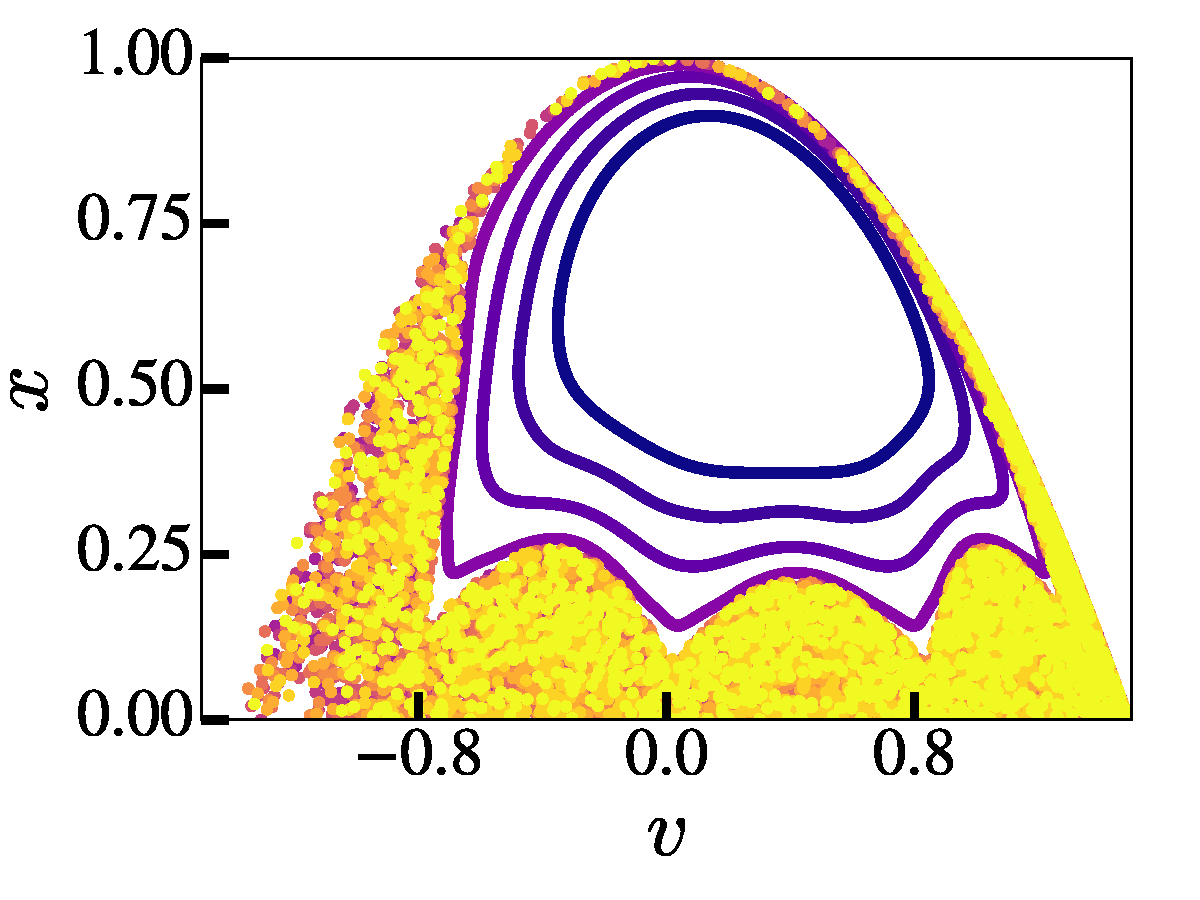
\includegraphics[width=0.8\linewidth]{multiple_r0_1_poincare}
  \caption{Poincare sections for 12 sets of initial conditions, varying $x_2$
  from $0.9$ to $1.08$ in even amounts, with $m_2/m_1 = 0.9$ and $v_1 = 0.879$.
  Darker colors indicate smaller values of $x_2$.}
  \label{fig:multiple}
\end{figure}

Interestingly, by varying $x_2$, we can see that the phase space
trajectories devolve from closed loops to a more chaotic structure. This is shown
in Fig.~\ref{fig:multiple}, where it is shown that setting $x_2$ near $x_1$
produces nonchaotic, closed trajectories through phase space, and by slowly raising
$x_2$, we begin to obtain more complex, chaotic behavior. This chaotic behavior
is further explored in the next section.


\subsubsection{Autocorrelation}\label{sec:9-acorr}

As before, calculating autocorrelation for these trajectories gives insight into
how chaotic the trajectories are.

\begin{figure}
  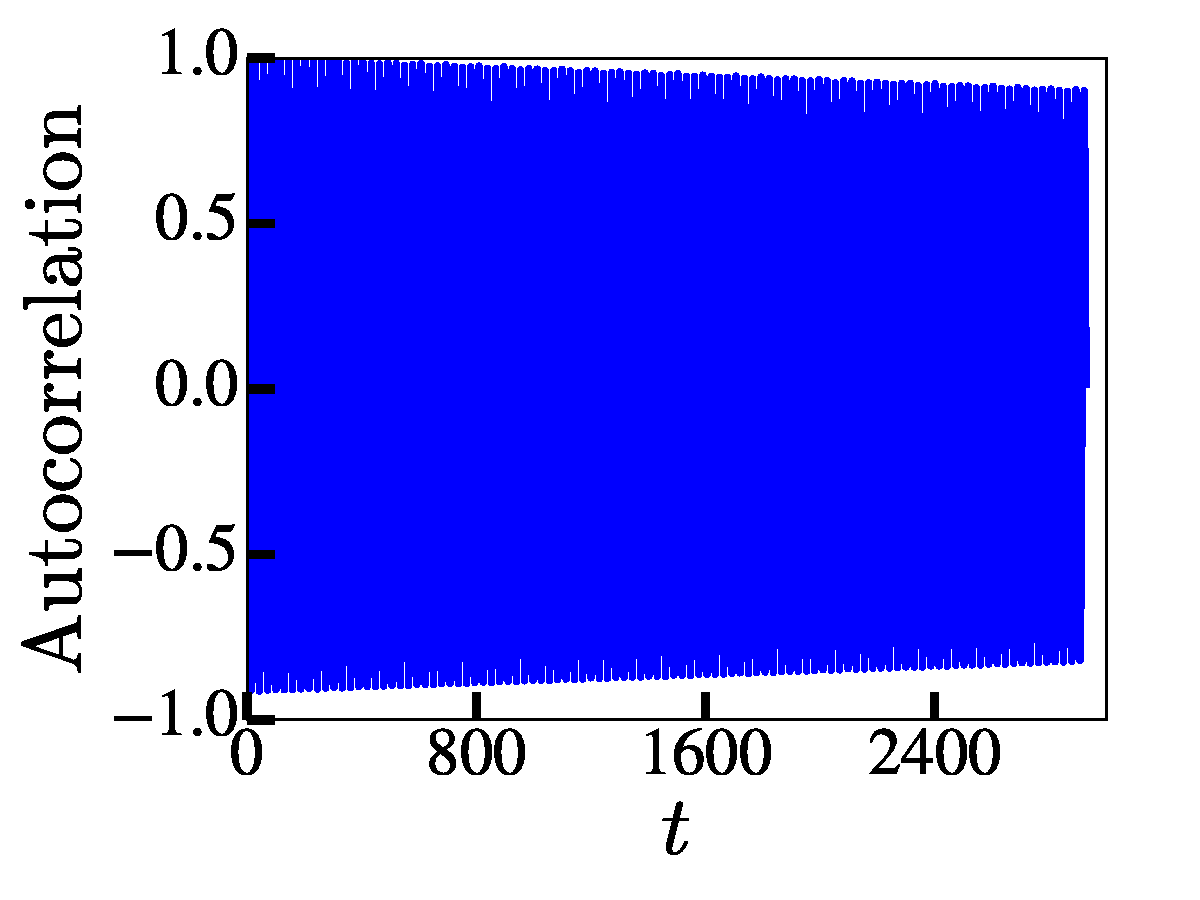
\includegraphics[width=0.8\linewidth]{nonchaotic_r0_1_acorr}
  \caption{Autocorrelation for $m_2/m_1 = 9$, with $v_1=0.879$. The autocorrelation
  rapidly oscillates, which causes it to appear almost solid. However, strong
  correlation is still present even at long times.}
  \label{fig:9-acorr-nonchaotic}
\end{figure}

For the case examined above, the autocorrelation is shown in Fig.~\ref{fig:9-acorr-nonchaotic}
over $t=0$ to $2930$. A strong correlation is observed throughout this time,
which is very long compared to the period of oscillations in the system. This
shows that the system is aperiodic despite how it looks over short, easily
visualizable timescales as in Fig.~\ref{fig:9-traj-nonchaotic}.


\subsubsection{Lyapunov Exponent}

We can further characterize how chaotic this motion is by examining separation
between two trajectories with very similar initial conditions. The separation
between the above system and an identical system with $x_2$ increased by $10^{-6}$
is shown in Fig.~\ref{fig:9-lyapunov-nonchaotic}.

\begin{figure}
  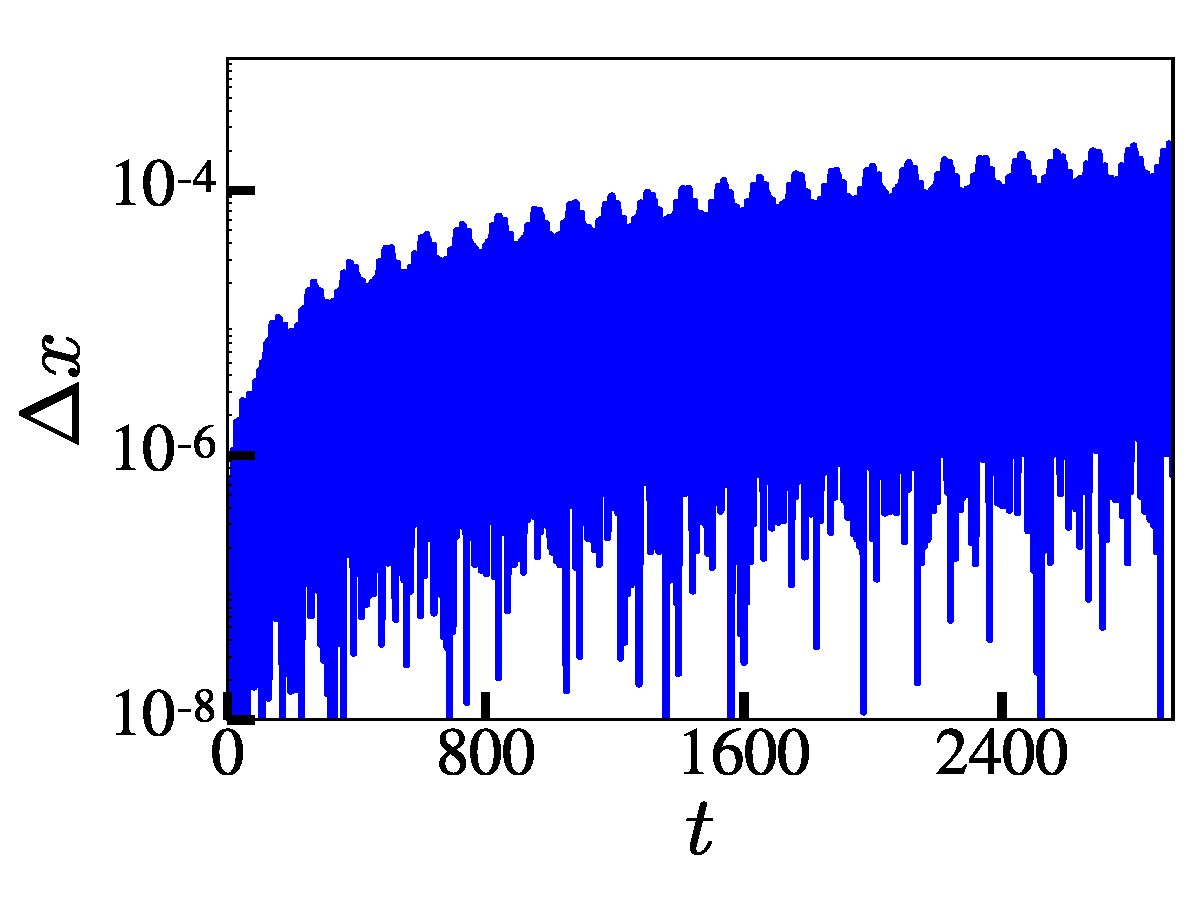
\includegraphics[width=0.8\linewidth]{nonchaotic_r0_1_lyapunov}
  \caption{Log plot of separation in ball 2 trajectories $\Delta x$
   between two systems for $m_2/m_1 = 9$ and $v_1=0.879$, with
  initial conditions differing by $10^{-6}$. Separation remains small, compared
  to the scale of the trajectories.}
  \label{fig:9-lyapunov-nonchaotic}
\end{figure}

Separation between the two is
nonzero, but grows extremely slowly over very large timescales relative to the
timescale of the balls' trajectories. The Lyapunov exponent, calculated as the slope
of this log plot, is positive but very small. This shows that the system is not
strongly sensitive to initial conditions, and therefore is only weakly chaotic
or not at all.





\subsection{Chaotic ($m_2/m_1 = 9$)}\label{sec:chaotic-9}

By setting
$v_1=0$ for the $m_2/m_1$ case, we can
once again get chaotic motion, shown in the trajectories and Poincare sections
in Fig.~\ref{fig:9-chaotic}.
By varying only the mass ratio and no other initial conditions from
Sec.~\ref{sec:nonchaotic}, the trajectories of the balls in Fig.~\ref{fig:9-traj}
now exhibit much more erratic trajectories than was seen previously for this
mass ratio in Fig.~\ref{sec:partially_chaotic}.

\begin{figure}
  \begin{subfigure}{0.8\linewidth}
    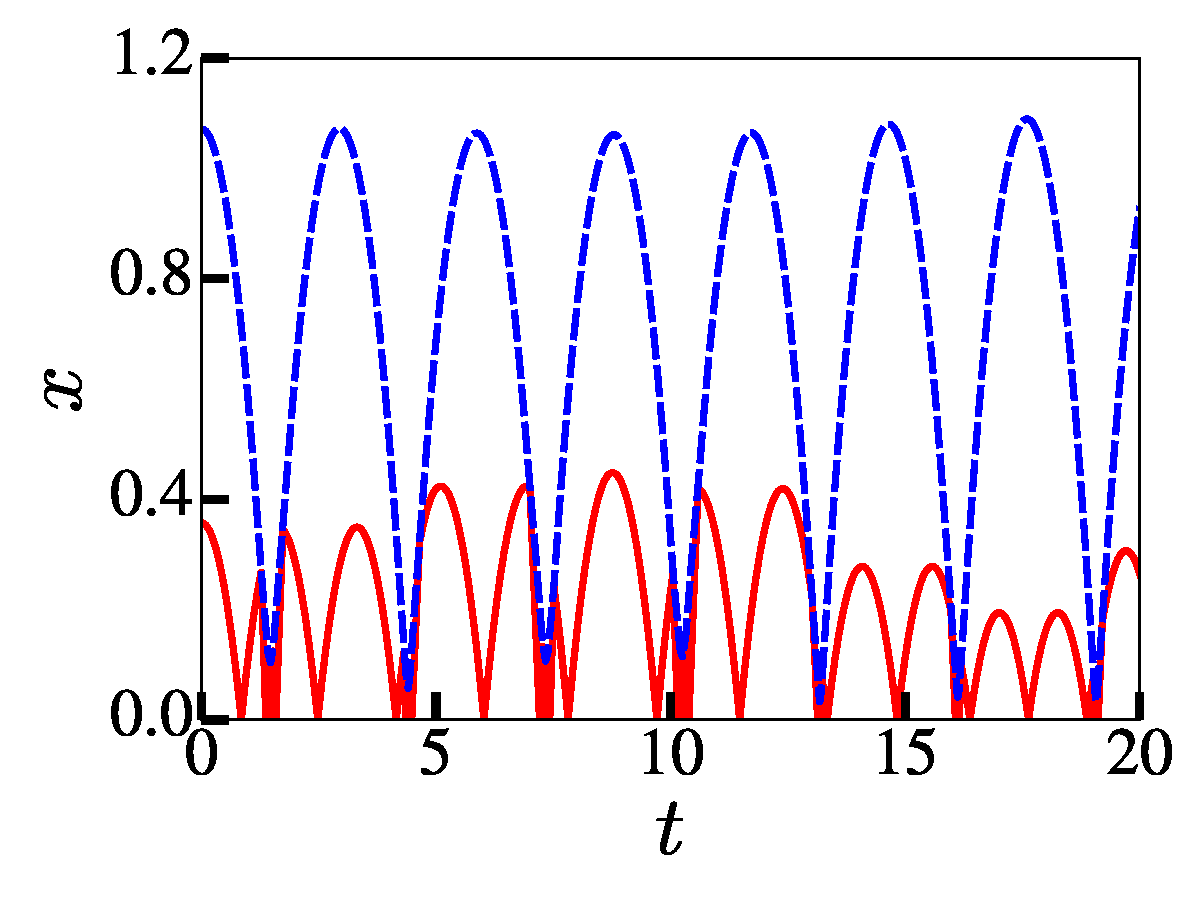
\includegraphics[width=\linewidth]{r0_1_traj}
    \caption{Trajectories of ball 1 (red, solid line) and ball 2 (blue, dashed line).
    Aperiodic motion is visible.}
    \label{fig:9-traj}
  \end{subfigure}

  \begin{subfigure}{\linewidth}
    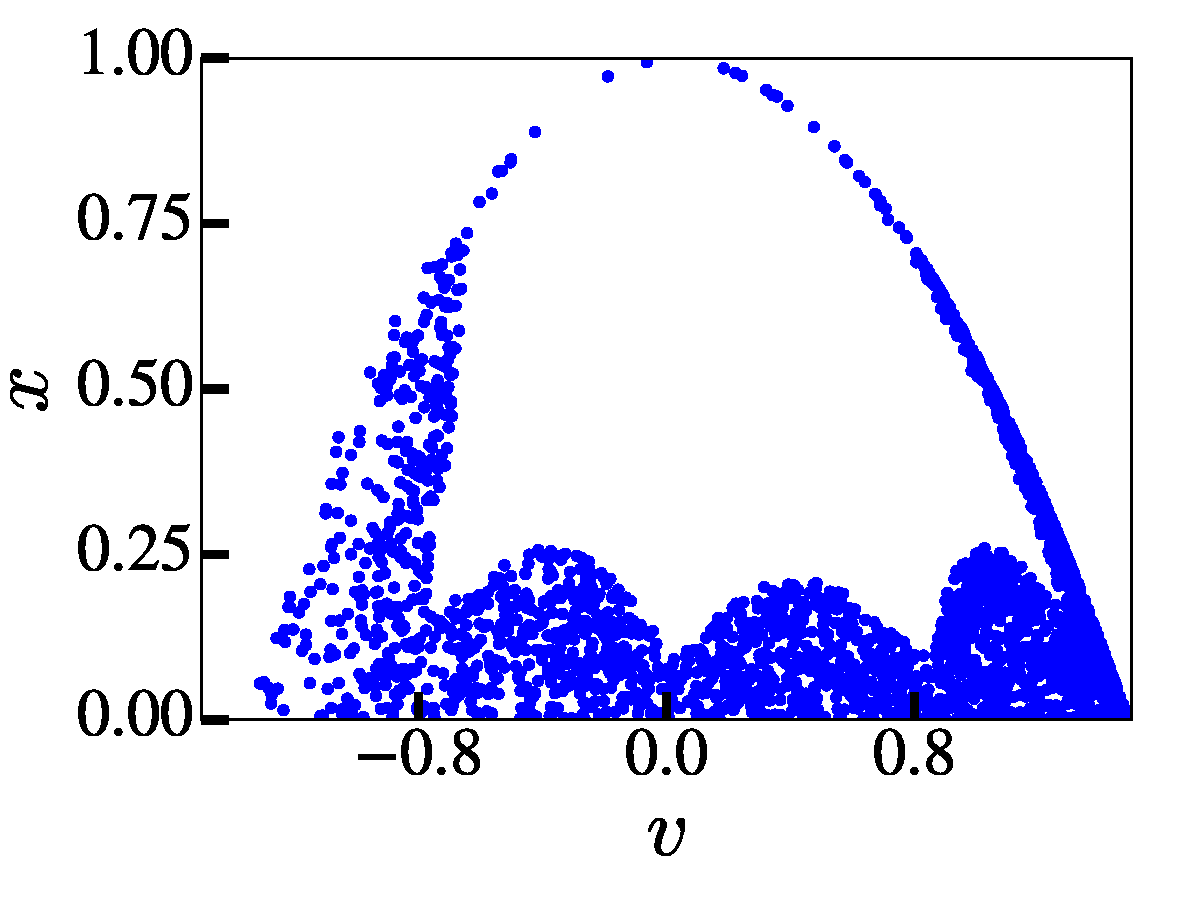
\includegraphics[width=0.8\linewidth]{r0_1_poincare}
    \caption{Poincare section for ball 2, plotted in phase space for every collision
    between the balls to $t=5000$s.}
    \label{fig:9-poincare}
  \end{subfigure}

  \caption{Trajectories and Poincare section for $m_2/m_1 = 9$, exhibiting
  aperiodic, chaotic behavior.}
  \label{fig:9-chaotic}
\end{figure}

Additionally, the Poincare section shown in Fig.~\ref{fig:9-poincare} grows
increasingly complex compared to Fig.~\ref{fig:1-poincare}. This indicates that
the balls are now sampling a much larger region in phase space, and therefore that
the trajectories of each period of motion have begun to vastly change between events.

\subsubsection{Autocorrelation}

As in Sec.~\ref{sec:9-acorr}, the autocorrelation of these trajectories is
analyzed in Fig.~\ref{fig:9-acorr}. Unlike the nonchaotic case shown in Fig.~\ref{fig:9-acorr-nonchaotic},
the autocorrelation
rapidly approaches zero, indicating the trajectories show little self-similarity.
This shows that the system is aperiodic.

\begin{figure}
    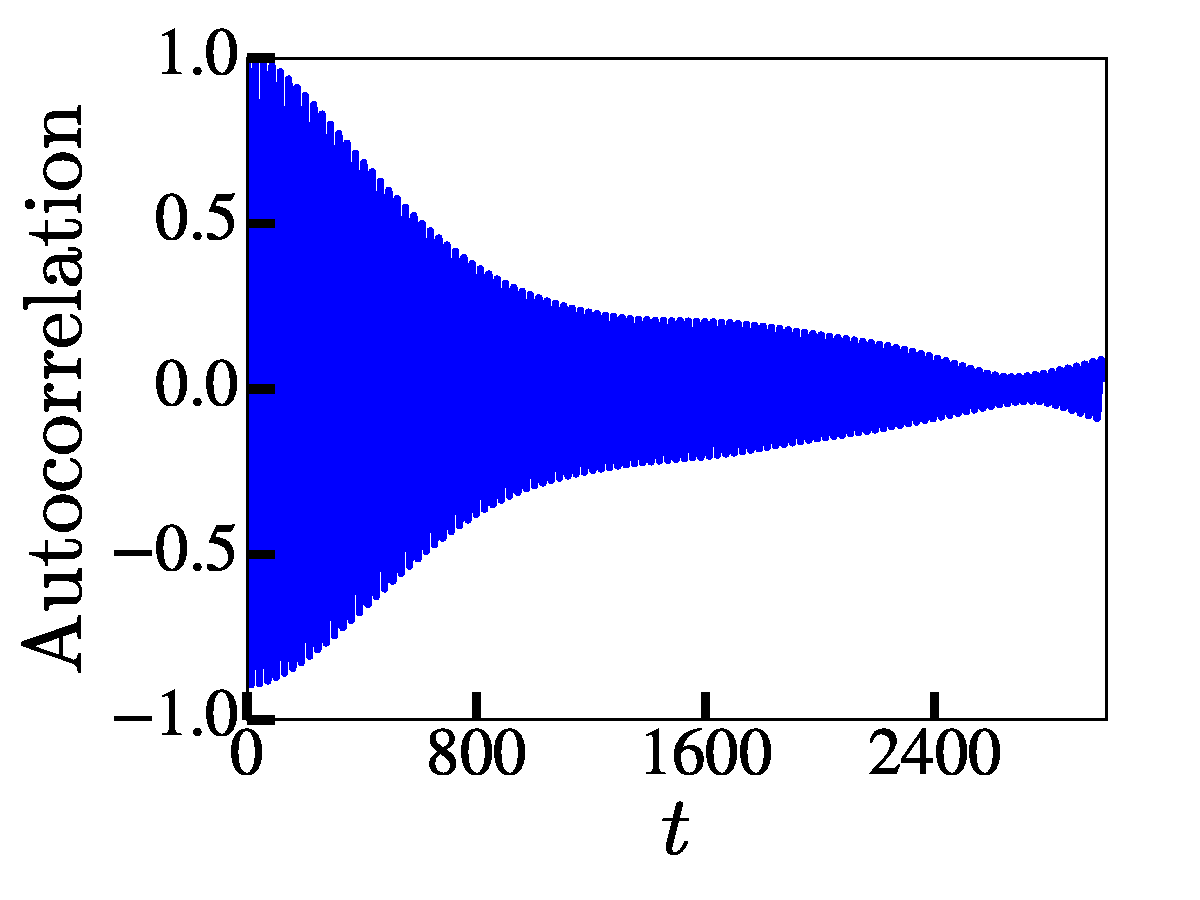
\includegraphics[width=0.8\linewidth]{r0_1_acorr}
    \caption{Autocorrelation for $m_2/m_1 = 9$, with $v_1=0$. The autocorrelation
    rapidly oscillates, causing it to appear almost solid. At long times,
    the autocorrelation approaches zero.}
    \label{fig:9-acorr}
\end{figure}

\subsubsection{Lyapunov Exponent}

Finally, we can verify the chaotic behavior in this system by comparing behavior
over time with slight variations in initial conditions. Once again two nearly identical
systems are run, except with $x_2$ varied by $10^{-6}$. However, in Fig.~\ref{fig:9-lyapunov}
it can be seen that the separation now extremely rapidly grows to order $1$, the same order
of the magnitude of the ball's trajectories.
The steep slope of the initial part of this plot
in Fig.~\ref{fig:9-lyapunov-zoomed} indicates a large positive Lyapunov exponent.
It is meaningful to consider this initial growth since the separation must cease
growing regardless of how chaotic the system is once it reaches the scale of the
balls' trajectories, as the balls cannot be separated by more than what their
maximum height is.
This shows that this system is extremely sensitive
to initial conditions, and confirms that it is chaotic.

\begin{figure}[h]
  \begin{subfigure}{\linewidth}
    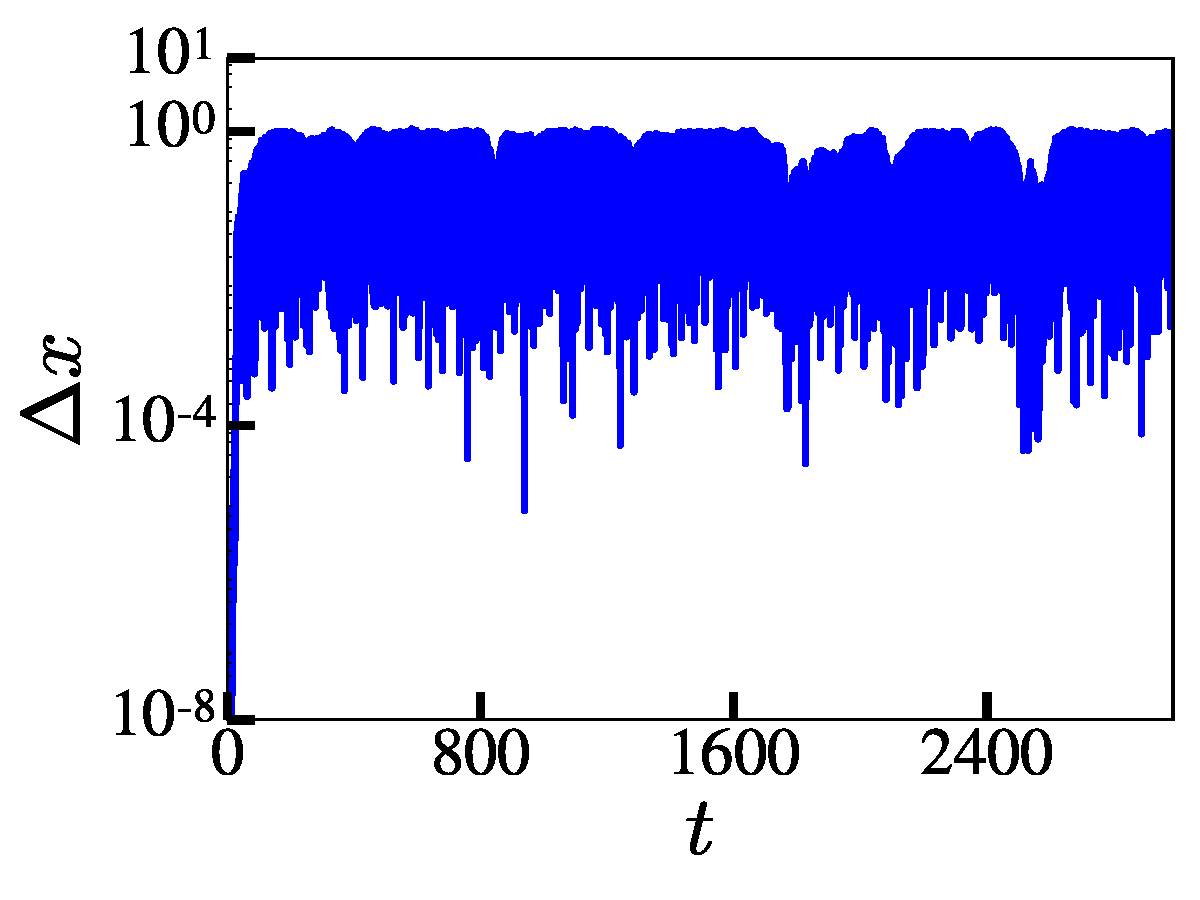
\includegraphics[width=0.8\linewidth]{r0_1_lyapunov}
    \caption{Long-term behavior over the entire duration of the simulation.
    Separation reaches and remains on the order of $1$.}
    \label{fig:9-lyapunov}
  \end{subfigure}

  \begin{subfigure}{0.8\linewidth}
    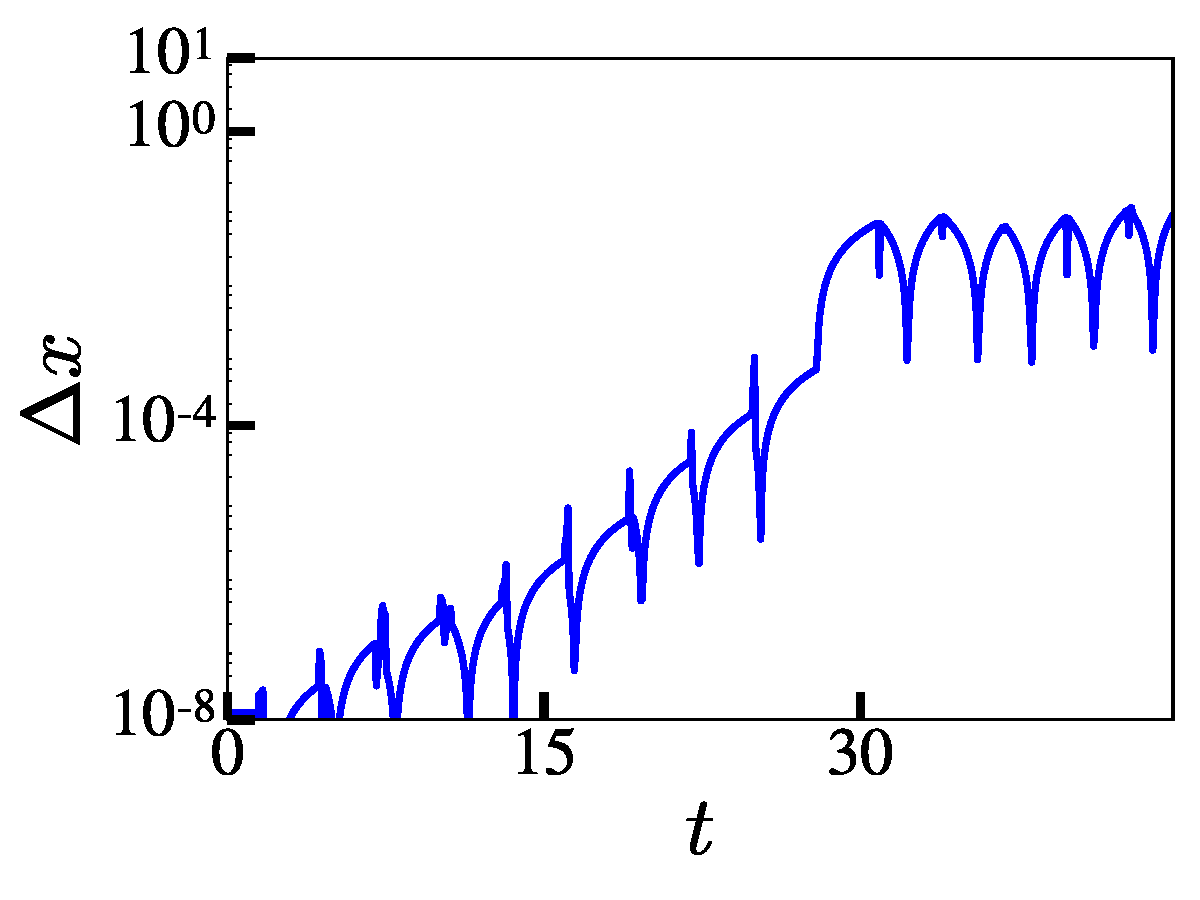
\includegraphics[width=\linewidth]{zoomed_r0_1_lyapunov}
    \caption{Zoomed in view of the above figure for short times, showing the
    exponential growth of the separation.}
    \label{fig:9-lyapunov-zoomed}
  \end{subfigure}

  \caption{Log plot of separation in ball 2 trajectories $\Delta x$
  between two systems for $m_2/m_1 = 9$ and
  $v_1=0$, with
  initial conditions differing by $10^{-6}$. Separation rapidly grows to order
  $10^0$, the order of the oscillations.}
\end{figure}



\subsection{Chaotic ($m_2/m_1 = 0.5$)}\label{sec:chaotic-2}
Chaotic behavior can also be observed for another mass ratio, $m_2/m_1 = 0.5$
Initial conditions are once more set to the original values of
$v_1 = v_2 = 0 \mathrm{m/s}$ and
$x_1 = 1$m, $x_2 = 3$m.

The trajectories for this system shown in
Fig.~\ref{fig:2-traj} appear aperiodic, with roughly similar structure but varying
amplitudes. This is confirmed by the analysis of the autocorrelation in Fig.~\ref{fig:2-acorr},
which shows a drop to 0 even quicker than that for $m_2/m_1$ in Fig.~\ref{fig:9-acorr}.


\begin{figure}
  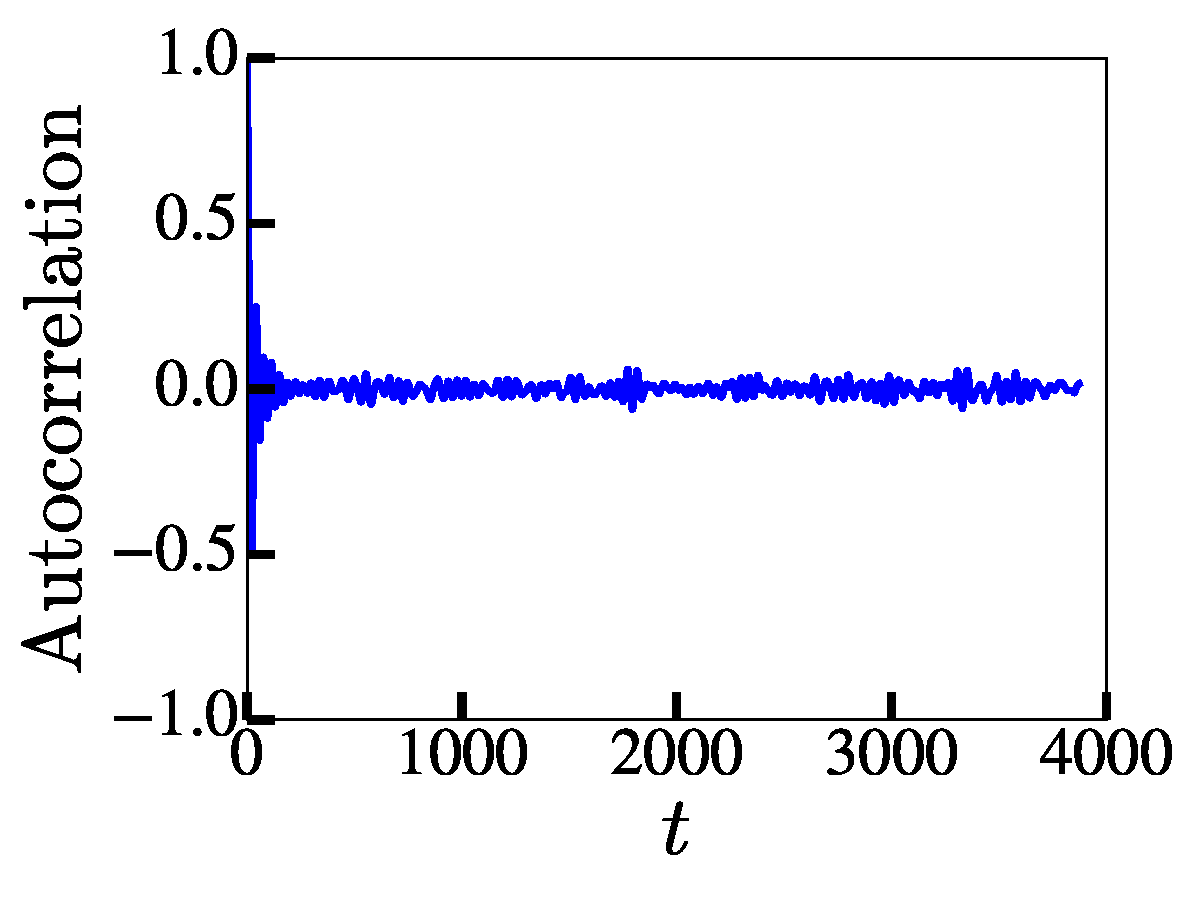
\includegraphics[width=0.8\linewidth]{r2_0_acorr}
  \caption{Autocorrelation for $m_2/m_1 = 0.5$. Autocorrelation rapidly reaches
  0 and oscillates about it, indicating strongly chaotic behavior.}
  \label{fig:2-acorr}
\end{figure}


The Poincare section for this system in Fig.~\ref{fig:2-poincare} again shows the
sampling of wide areas of phase space that do not lie along a closed trajectory
consistent with chaotic motion.

\begin{figure}
  \begin{subfigure}{0.8\linewidth}
    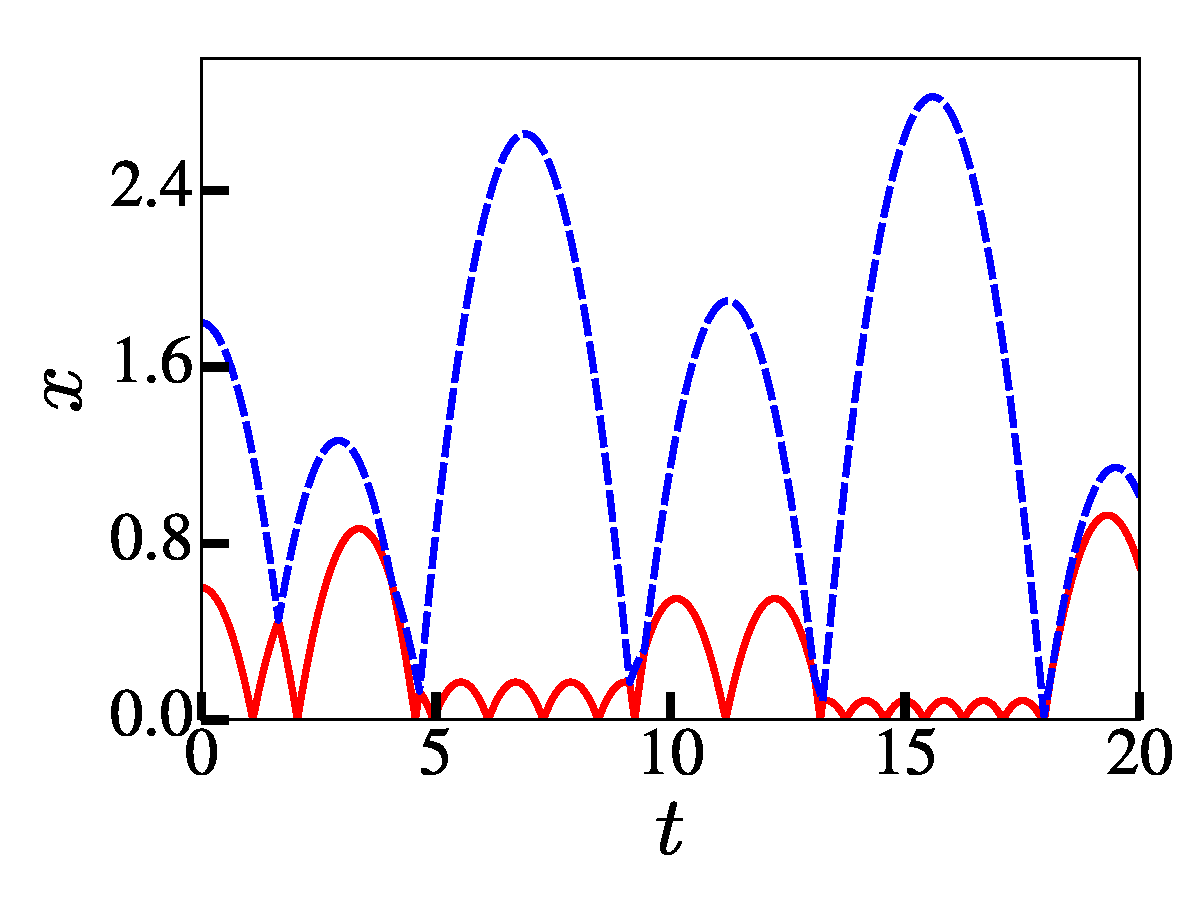
\includegraphics[width=\linewidth]{r2_0_traj}
    \caption{Trajectories of ball 1 (red, solid line) and ball 2 (blue, dashed line).
    Aperiodic motion is visible.}
    \label{fig:2-traj}
  \end{subfigure}

  \begin{subfigure}{0.8\linewidth}
    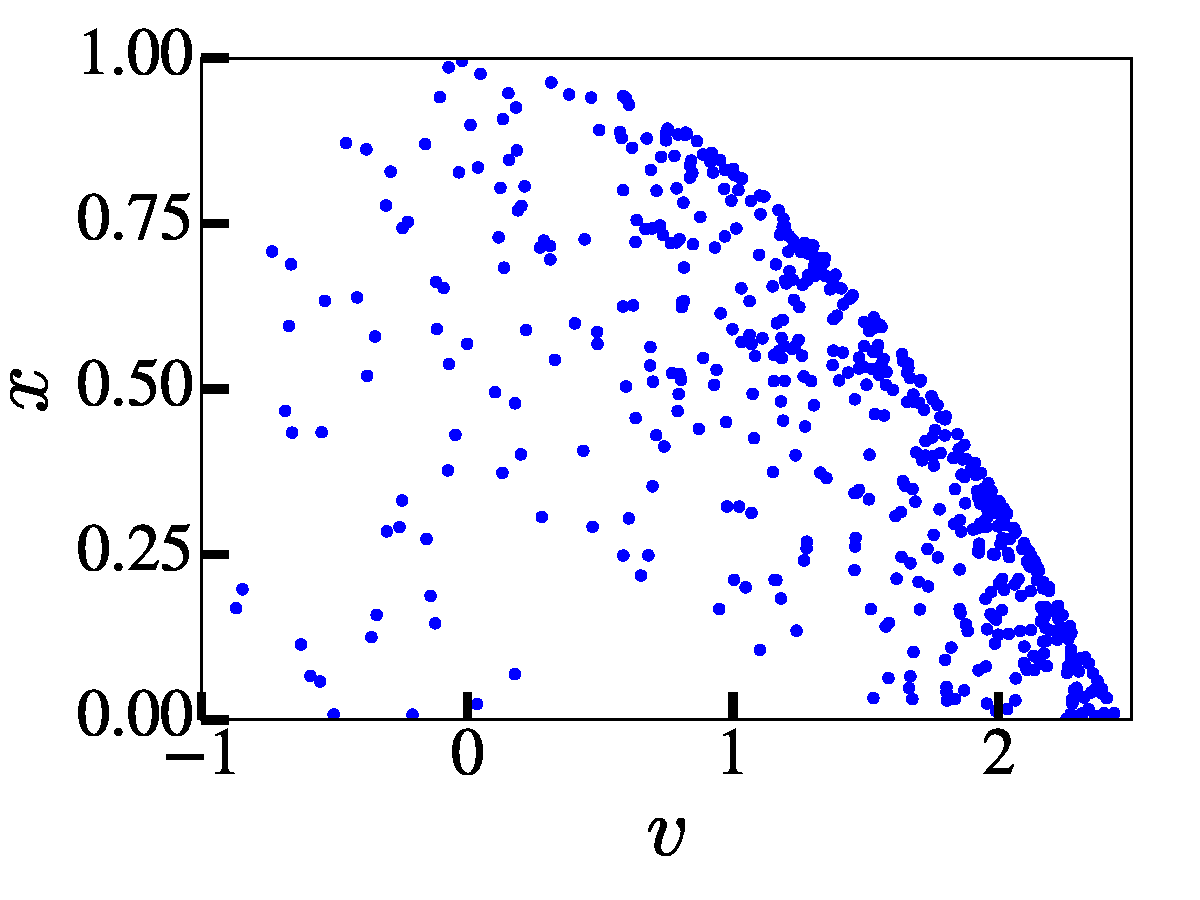
\includegraphics[width=\linewidth]{r2_0_poincare}
    \caption{Poincare section for ball 2, plotted in phase space for every collision
    between the balls to $t=5000$s.}
    \label{fig:2-poincare}
  \end{subfigure}

  \caption{Trajectories and Poincare section for $m_2/m_1 = 0.5$.}
\end{figure}

\begin{figure}
  \begin{subfigure}{\linewidth}
    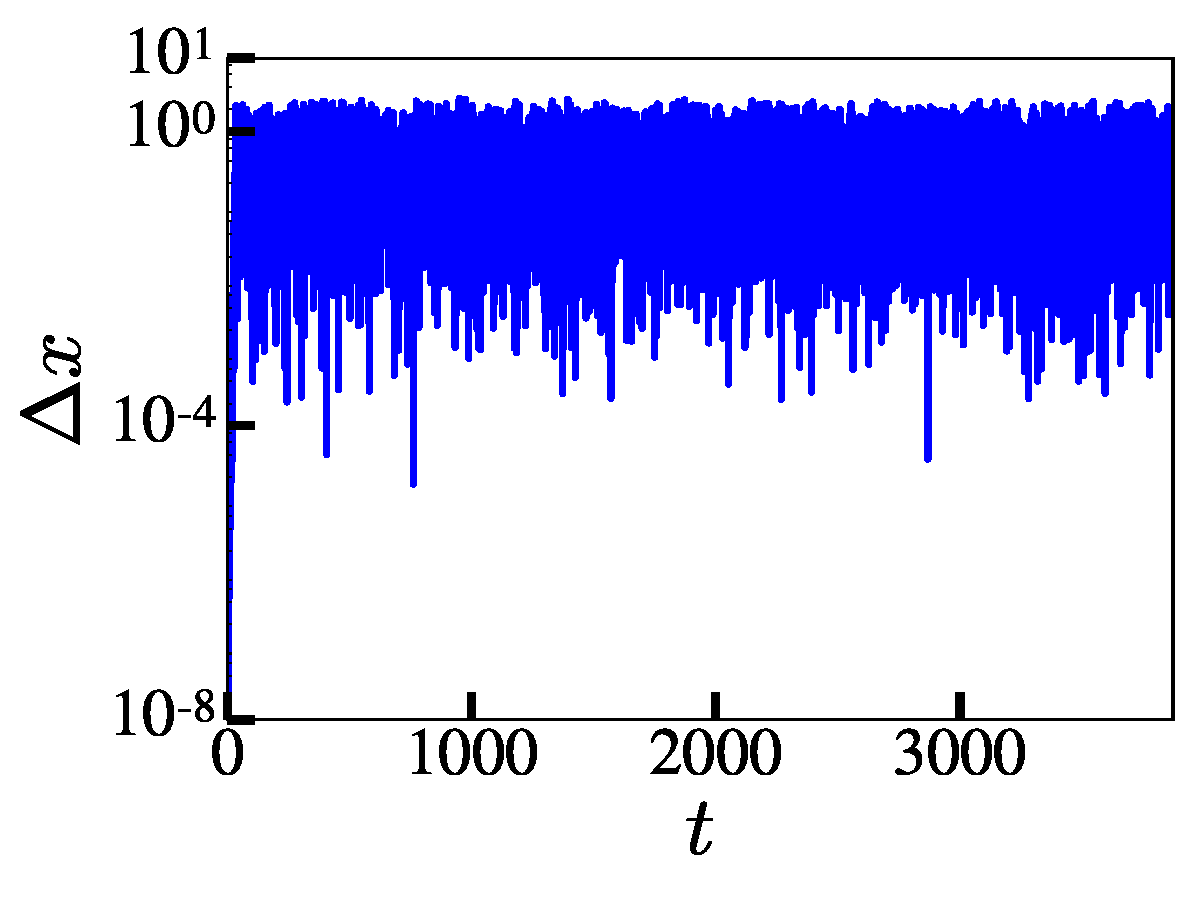
\includegraphics[width=0.8\linewidth]{r2_0_lyapunov}
    \caption{Long-term behavior over the entire duration of the simulation.
    Separation reaches and remains on the order of $1$.}
    \label{fig:2-lyapunov}
  \end{subfigure}

  \begin{subfigure}{0.8\linewidth}
    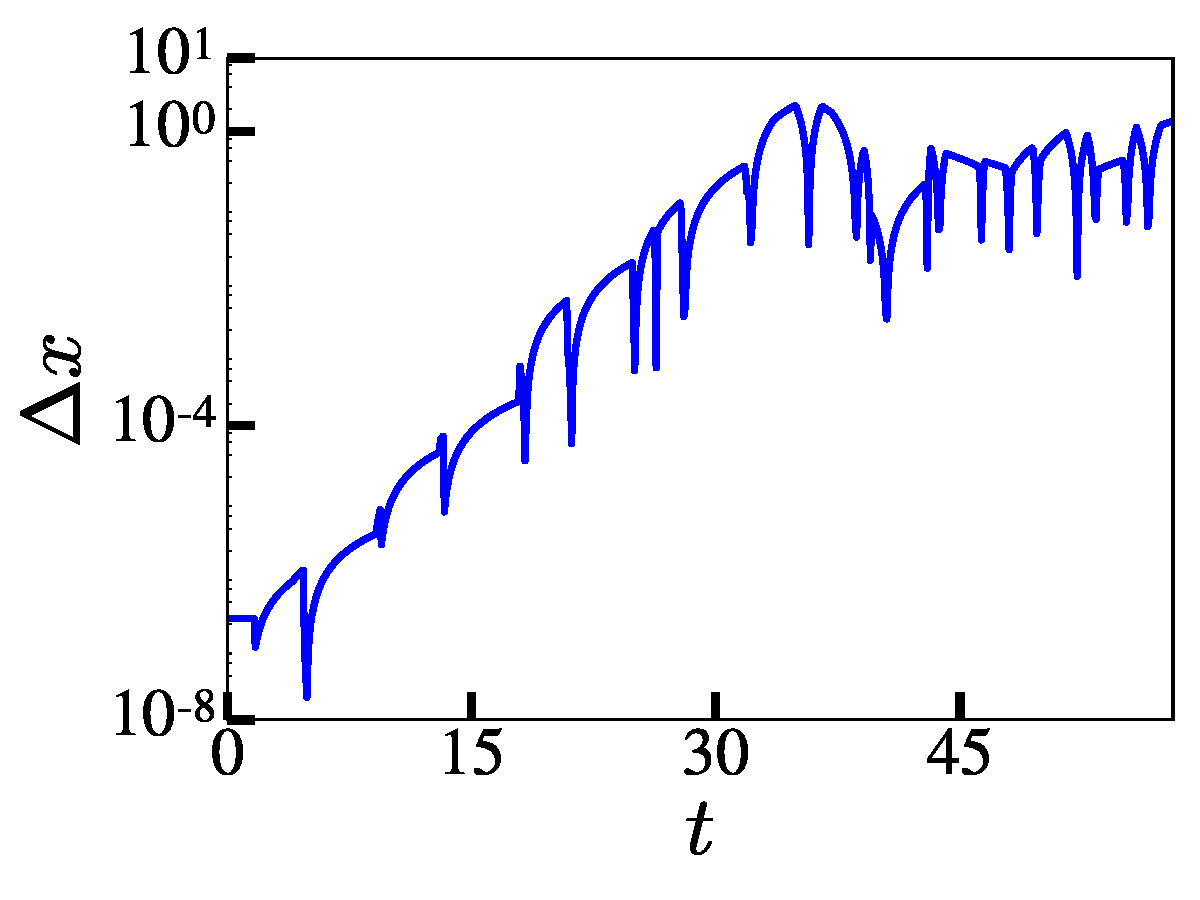
\includegraphics[width=\linewidth]{zoomed_r2_0_lyapunov}
    \caption{Zoomed in view of the above figure for short times, showing the
    exponential growth of the separation.}
    \label{fig:2-lyapunov-zoomed}
  \end{subfigure}
  \caption{Log plot of separation in ball 2 trajectories $\Delta x$
   between two systems with $m_2/m_1 = 0.5$, with $x_2$ varied by $10^{-6}$.
   The separation approaches the order of the ball's oscillations.}
\end{figure}

Finally, separation in time for two systems with slightly varied initial conditions
again rapidly approaches the order of the trajectories, as seen in Fig.~\ref{fig:2-lyapunov}.
This is more clearly seen for the initial times where the separation is growing
in Fig.~\ref{fig:2-lyapunov-zoomed}.
This means the Lyapunov exponent is positive, and that the system is therefore
chaotic.

This combination of factors indicates that this system is indeed chaotic, and in
fact converges to chaotic behavior even faster than the system analyzed in the
previous section.





\section{Conclusions} \label{sec:conclusion}

In this paper, a system of two colliding balls in one dimension was studied.
Different mass ratios and initial velocities and positions were explored to
examine the onset of chaotic motion.

In Section~\ref{sec:nonchaotic}, the mass ratio of balls 1 and 2 was set to
$m_1/m_2=1$. The initial positions of the balls were set to $x_1 = 1\mathrm{m}$
and $x_2=3\mathrm{m}$.Periodic motion was shown in the trajectories, and a well-defined
trajectory through phase space was demonstrated in a Poincare section plotted for
ball 2 at the time of each collision. Analysis of the autocorrelation function
showed strong correlation even at long times compared to the timescale of events
in the system, indicating periodic, nonchaotic motion.

In Section~\ref{sec:partially_chaotic}, the mass ratio of the balls was set to
$m_1/m_2 = 9$, and the velocity of ball 1 $v_1$ was set to $1.5 \mathrm{m/s}$.
Though the trajectories appeared more complex, the autocorrelation again showed
strong correlation at long times. The Poincare section for ball 2 also showed
more complex structure, but still followed a well-defined trajectory through
phase space. Analyzing the separation in position between ball 2 in two systems
with $x_2$ varied by $10^-6$ showed separations on the order of $10^{-4}$, much
smaller than the amplitude of the balls' oscillations.

However, varying the initial position of ball 1 $x_1$ revealed
Poincare sections that transitioned from following these well-defined trajectories
to sampling wide areas of phase space. This was the first suggestion of chaotic
behavior in the system.

In Section~\ref{sec:chaotic-9}, the mass ratio was left at $m_2/m_1=9$, but the
initial velocity $v_1$ was reset to $0$. This system exhibited aperiodic trajectories
along with a Poincare section showing $x_2$ widely sampling phase space without
following any particular trajectory. This suggested chaotic behavior, which was
confirmed by an autocorrelation that approached 0.

Additionally, the separation
of ball 2 in two systems with $x_2$ varied by a small amount, $10^{-6}$, showed
that separation rapidly approached the order of the trajectories.
This strong sensitivity to initial conditions is a hallmark of chaotic behavior.

Finally, a strongly chaotic system was analyzed in Section~\ref{sec:chaotic-2}
by changing the mass ratio to $m_s/m_1=0.5$. Again the trajectories exhibited
aperiodic motion, verified by an autocorrelation that approached 0 even faster
than in the previous section. The Poincare section showed ball 2 exploring a wide
region of phase space that once more did not follow a consistent trajectory.
Sensitivity to initial conditions was demonstrated by the separation between two
systems with similar initial conditions rapidly approaching the order of the positions.

These findings demonstrate that even a relatively simple system can exhibit a wide
range of dynamical behaviors. Slight variations in initial conditions can cause
dramatic changes in behavior, causing the system to shift from fairly simple
periodic motion to following determininistic, but highly complex trajectories.

\subsection{Future Work}

The algorithm used for these simulations could be considerably optimized by
implementing parallelization. Generating the functions which determine motion in
the intervals between events is a fairly computationally cheap task. Once this
has been performed, all the data to determine the position of a ball at any point
in time has been fully defined. So, sampling the datapoints in time along these
trajectories could be split across multiple cores.

In fact, having defined the
trajectory computations as lambda functions facilitates use of Python's built in
multiprocessing module, which allows mapping functions across an arbitrary number
of threads. This would optimally be set to the number of cores available on the
system.

Implementing multiprocessing in this manner would result in a significant
speedup in running the algorithm as-is. Nominally, this should linearly increase
the run-time of the trajectory sampling with the numer of cores available. This
would allow sampling of much longer trajectories.

Generating more detailed Poincare sections for larger numbers could be improved
in a similar manner. Currently, the multiple Poincare sections plotted in
Fig.~\ref{fig:multiple} are generated sequentially. This imposes a practical
limitation on the number of events that can be sampled for each Poincare section,
since the time to generate all of them increases linearly with the number of Poincare
sections generated. If these were generated in parallel, this bottleneck would be
removed, and one could generate as many Poincare sections as cores available in
the same amount of time as one.

Finally, I believe a functional implementation of the simulation code in Haskell
would also provide a significant speedup, particularly in the trajectory sampling.
The current code involves generating and manipulating large arrays of data.
Haskell's lazy evaluation could significantly speed this up, since values would
not be generated until actually needed for a calculation. This eliminates some
of the interrim array manipulation that is done between generating the initial
phase space coordinates of events and actually using them to generate positions
of the balls during the intervals between events.



\FloatBarrier
\begin{thebibliography}{1}
\bibitem{taylor}
  Taylor, J. R. (2005).
  \textit{Classical mechanics}.
  Sausalito, CA: University Science Books.

\bibitem{whelan}
Whelan, N. D., Goodings, D. A. \& Cannizzo, J. K. (1990).
Two balls in one dimension with gravity.
\textit{Phys. Rev. A}, 42, 742-754.


\bibitem{assignment}
M. Shay.
\textit{Deterministic Chaos in Classical 1D Scattering}.
(University of Delaware, Spring 2018)

\end{thebibliography}

\clearpage
\appendix
\section{Trajectory Algorithm}\label{appendix:traj}
In creating the algorithm for sampling ball trajectories at evenly-spaced times,
a few computational optimizations were made to optimize runtime.

A general overview of the algorithm is provided in Section~\ref{sec:methods}.
Each interval between events corresponds to a list element which is itself a list
of \texttt{[start\_time,~end\_time,~x\_func,~v\_func]}, where \texttt{start\_time}
and \texttt{end\_time} are the start and end times of that interval, and
\texttt{x\_func} and \texttt{v\_func} are lambda functions that return the
position and velocity of the ball at some time since the previous interval. A
list of lists is created for each ball.

This method was originally chosen to work with NumPy's \texttt{piecewise()}
function, which as the name suggests will piecewise evaluate a list of functions
over a list of input values according to a matrix of boolean values that specifies
when each function is valid for each input. However, generating this boolean matrix
was a slow task, and the boolean matrix has dimension
[sampled~times~$\times$~number~of~events].
This matrix rapidly grows extremely large, and becomes very slow to manipulate.

Instead, a simpler solution was found by exploiting the fact that the lists of
intervals are already in sequential order. As the timesteps are iterated over,
the first element of the list of intervals is used. Once the time being sampled
is larger than the end time of that interval, the sub-list corresponding to that
element is removed from the list of intervals, and the first element in the list
of intervals becomes the next interval. This avoids usage of \texttt{piecewise()}
entirely.

A side effect of this method is that no form of array searching to find the
appropriate interval to evaluate the function over is necessary - only the first
element is ever used.


\end{document}
